\documentclass[12pt,a4paper]{article}
\usepackage{amsmath,amssymb,amsbsy,amsfonts}
\usepackage{graphicx}
\usepackage{float}
\usepackage{geometry}
\usepackage{booktabs}
\usepackage{caption}
\usepackage{enumitem}
\usepackage{setspace}
\usepackage{hyperref}
\usepackage{CJKutf8}

\geometry{a4paper, left=2.5cm, right=2.5cm, top=2.5cm, bottom=2.5cm}
\onehalfspacing
\renewcommand{\baselinestretch}{1.5}

\begin{document}

\begin{CJK}{UTF8}{gkai}

\begin{center}
{\fontsize{16pt}{18pt}\selectfont\textbf{碳化硅外延层厚度的确定}}\\[8pt]
{\fontsize{14pt}{16pt}\selectfont\textbf{Determination of Silicon Carbide Epilayer Thickness}}\\[15pt]
{\fontsize{12pt}{14pt}\selectfont\textbf{摘要}}\\[5pt]
\end{center}

\noindent
碳化硅作为第三代半导体材料，其外延层厚度是影响器件性能的关键参数。本文基于红外干涉法，建立了双光束干涉和多光束干涉的数学模型，提出了多种厚度确定算法，包括相邻极值法、线性回归法、FFT法和差分进化拟合法。研究表明，SiC材料的多光束干涉效应极小（显著性参数$\beta\approx0.001$），双光束近似完全可靠；而Si材料在高掺杂衬底情况下多光束干涉显著（$\beta>0.2$），必须采用多光束模型，否则厚度测量误差约为0.5\%。通过差分进化算法进行全局优化，有效避免了局部最优问题，提高了厚度测量精度。

\vspace{8pt}

\noindent
{\textbf{关键词：}} 碳化硅；外延层厚度；红外干涉法；多光束干涉；差分进化算法

\vspace{15pt}

\section{引言}

碳化硅（SiC）作为一种新兴的第三代半导体材料，以其优异的物理化学性能，如宽禁带、高击穿电场、高热导率和高电子饱和漂移速度等，在功率器件、高频器件和高温器件领域具有广阔的应用前景\cite{1}。外延层厚度是SiC外延材料的关键参数之一，直接影响器件的击穿电压、导通电阻和频率特性。因此，建立一套科学、准确、可靠的外延层厚度测试方法具有重要的理论和实际意义。

红外干涉法是一种非破坏性的厚度测量方法，其基本原理是利用红外光在外延层与衬底界面反射产生的干涉条纹来确定厚度\cite{2}。该方法具有测量精度高、操作简便、不损伤样品等优点，已广泛应用于半导体外延层厚度的测量。

本文围绕SiC外延层厚度的确定问题，开展了以下研究工作：

\begin{enumerate}[label=\arabic*.]
\item 建立了双光束干涉条件下确定外延层厚度的数学模型；
\item 设计了多种厚度确定算法，并对SiC晶圆片的实测数据进行了分析；
\item 推导了多光束干涉的必要条件，分析了其对厚度计算精度的影响，并对Si晶圆片数据进行了处理。
\end{enumerate}

\section{基本假设与符号说明}

\subsection{基本假设}

为简化问题分析，本文作出以下基本假设：

\begin{enumerate}[label=(\arabic*)]
\item 红外光为单色平面波，在介质中传播时无吸收损耗；
\item 外延层为均匀、各向同性介质，厚度均匀；
\item 入射光为非偏振光，反射率取s偏振和p偏振的平均值；
\item 界面为理想光滑平面，反射和透射符合菲涅尔公式。
\end{enumerate}

\subsection{符号说明}

本文所用主要符号及其含义如表1所示。

\begin{table}[H]
\centering
\caption{主要符号说明}
\begin{tabular}{cl}
\toprule
符号 & 含义 \\
\midrule
$d$ & 外延层厚度（m） \\
$n_0$ & 空气折射率（$n_0=1$） \\
$n_1$ & 外延层折射率 \\
$n_2$ & 衬底折射率 \\
$\theta_0$ & 入射角（rad） \\
$\theta_1$ & 外延层内折射角（rad） \\
$\nu$ & 波数（cm$^{-1}$） \\
$\lambda$ & 波长（m） \\
$R$ & 反射率（\%） \\
$\beta$ & 多光束显著性参数 \\
$N$ & 掺杂浓度（cm$^{-3}$） \\
$m$ & 干涉级次 \\
\bottomrule
\end{tabular}
\end{table}

\section{双光束干涉模型}

\subsection{物理模型}

考虑三层介质结构：空气（折射率$n_0=1$）、外延层（折射率$n_1$，厚度$d$）、衬底（折射率$n_2$）。如图1所示，入射光在外延层上表面和下表面发生反射，两束反射光产生干涉现象。

\begin{figure}[H]
\centering
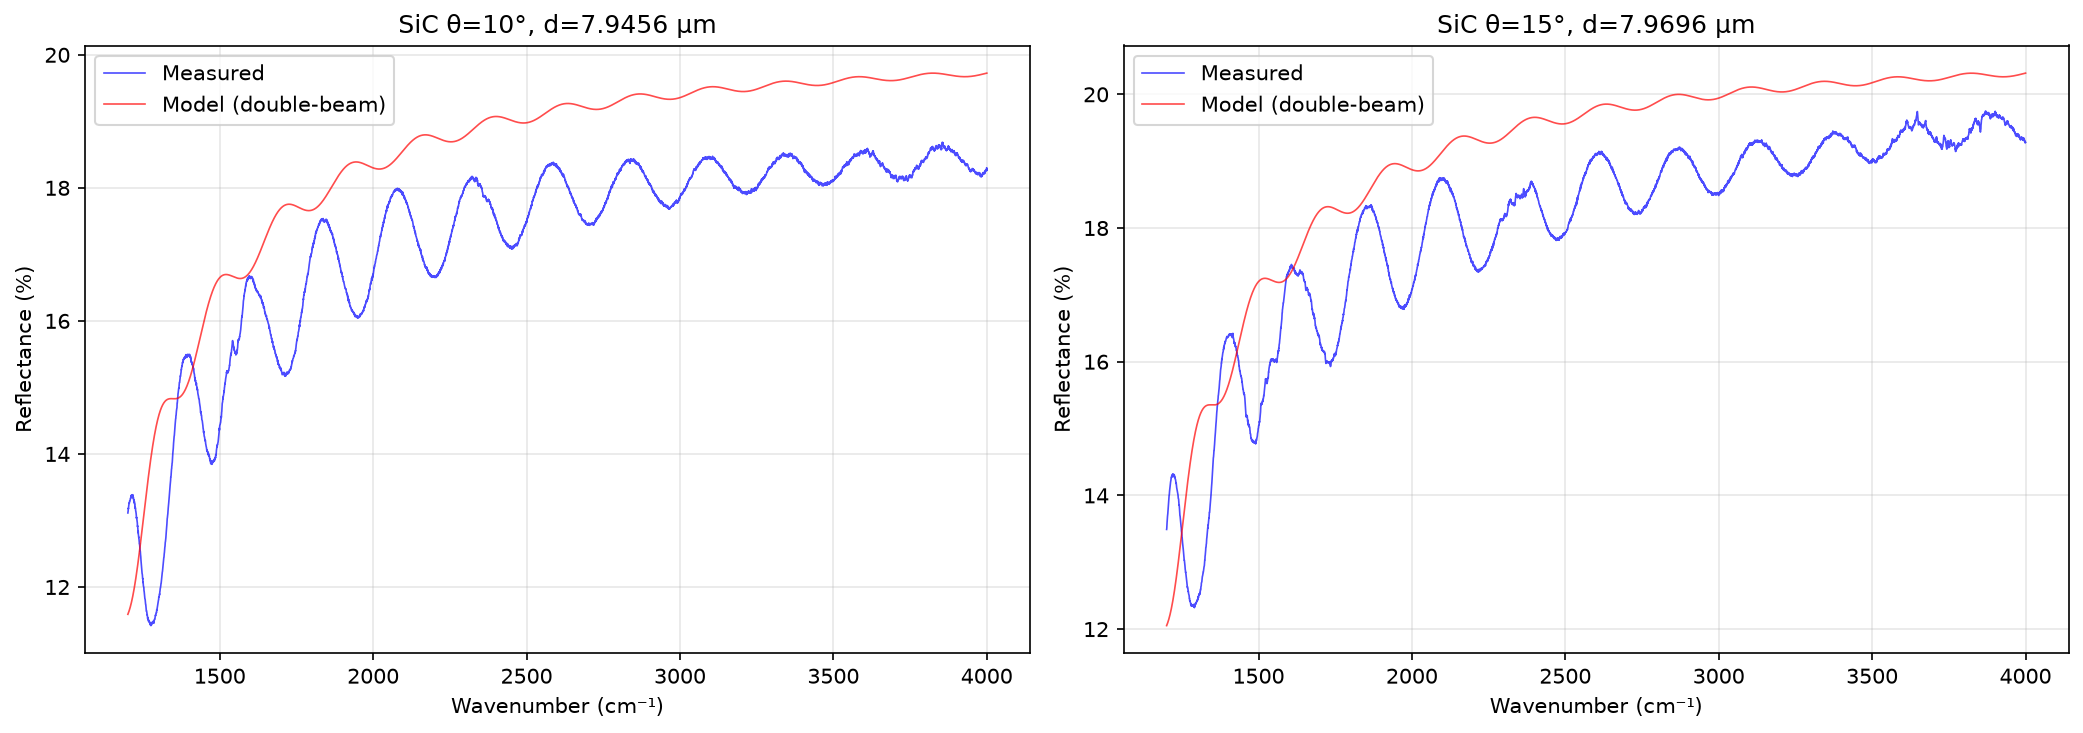
\includegraphics[width=0.6\textwidth]{q1_model_validation.png}
\caption{双光束干涉原理示意图}
\label{fig:double_beam}
\end{figure}

\subsection{光程差与相位差}

两束反射光的光程差为：

\begin{equation}
\Delta = 2n_1d\cos\theta_1
\end{equation}

其中$\theta_1$为外延层内的折射角，由斯涅尔定律可得：

\begin{equation}
\sin\theta_1 = \frac{n_0}{n_1}\sin\theta_0
\end{equation}

因此，$\cos\theta_1 = \sqrt{1 - \left(\frac{n_0}{n_1}\sin\theta_0\right)^2}$。

相位差$\delta$为：

\begin{equation}
\delta = \frac{2\pi}{\lambda} \cdot 2n_1d\cos\theta_1 = \frac{4\pi n_1d\cos\theta_1}{\lambda}
\end{equation}

考虑波数$\nu = 1/\lambda$（单位：cm$^{-1}$），则相位差可表示为：

\begin{equation}
\delta = 4\pi n_1d\cos\theta_1 \cdot \nu \times 10^{-2}
\end{equation}

\subsection{反射率公式}

根据菲涅尔公式，s偏振和p偏振的反射系数分别为：

\begin{align}
r_{01s} &= \frac{n_0\cos\theta_0 - n_1\cos\theta_1}{n_0\cos\theta_0 + n_1\cos\theta_1} \\
r_{01p} &= \frac{n_1\cos\theta_1 - n_0\cos\theta_0}{n_1\cos\theta_1 + n_0\cos\theta_0} \\
r_{12s} &= \frac{n_1\cos\theta_1 - n_2\cos\theta_2}{n_1\cos\theta_1 + n_2\cos\theta_2} \\
r_{12p} &= \frac{n_2\cos\theta_2 - n_1\cos\theta_1}{n_2\cos\theta_2 + n_1\cos\theta_1}
\end{align}

其中$\theta_2$为衬底内的折射角，满足$\sin\theta_2 = (n_0/n_2)\sin\theta_0$。

考虑界面反射的相位变化，双光束干涉的反射率为：

\begin{equation}
R = \frac{r_{01}^2 + r_{12}^2 + 2r_{01}r_{12}\cos(\delta + \phi)}{1 + r_{01}^2r_{12}^2 + 2r_{01}r_{12}\cos(\delta + \phi)}
\end{equation}

其中$\phi$为反射时的相位突变。对于非偏振光，取s偏振和p偏振的平均值：

\begin{equation}
R = \frac{R_s + R_p}{2}
\end{equation}

\section{折射率模型}

半导体材料的折射率随波长和掺杂浓度变化，采用Lorentz-Drude模型描述：

\begin{equation}
n(\nu) = \sqrt{\varepsilon_\infty + \sum_{j=1}^{m}\frac{A_j\nu_{Lj}^2}{\nu_{Lj}^2 - \nu^2 - i\Gamma_j\nu} - \frac{f\nu_p^2}{\nu^2 + i\gamma\nu}}
\end{equation}

其中$\varepsilon_\infty$为高频介电常数，$A_j$、$\nu_{Lj}$、$\Gamma_j$为Lorentz振子参数，$f$、$\nu_p$、$\gamma$为自由载流子参数。

自由载流子等离子体频率$\nu_p$与掺杂浓度$N$的关系为：

\begin{equation}
\nu_p^2 = \frac{Ne^2}{4\pi^2\varepsilon_0m^*c^2}
\end{equation}

其中$e$为电子电荷，$\varepsilon_0$为真空介电常数，$m^*$为有效质量，$c$为光速。

\section{厚度确定算法}

\subsection{相邻极值法}

干涉条纹的极大值和极小值满足以下条件：

\begin{align}
\text{极大值：} \quad 2n_1d\cos\theta_1 = m\lambda \\
\text{极小值：} \quad 2n_1d\cos\theta_1 = \left(m + \frac{1}{2}\right)\lambda
\end{align}

其中$m$为干涉级次。利用相邻两个极大值（或极小值）的波数$\nu_1$和$\nu_2$，可得：

\begin{equation}
d = \frac{1}{2\left[n_1(\nu_2)\cos\theta_1(\nu_2)\nu_2 - n_1(\nu_1)\cos\theta_1(\nu_1)\nu_1\right] \times 10^{-2}}
\end{equation}

\subsection{线性回归法}

定义光学厚度$OP(\nu) = n_1(\nu)\cos\theta_1(\nu)\nu$，则极大值条件可表示为：

\begin{equation}
OP(\nu) = \frac{m}{2d}
\end{equation}

对$OP(\nu)$与干涉级次$m$进行线性拟合，斜率为$\frac{1}{2d}$，从而求得厚度$d$。

\subsection{FFT法}

对反射率谱进行傅里叶变换，提取主频$f_d$，则厚度为：

\begin{equation}
d = \frac{f_d}{2n_{\text{ref}}\cos\theta_1}
\end{equation}

其中$n_{\text{ref}}$为参考折射率。

\subsection{差分进化拟合法}

采用差分进化算法对厚度$d$和掺杂浓度$N$进行全局优化，目标函数为：

\begin{equation}
\min_{d,N} \sum_{i=1}^{n} \left[R_{\text{meas}}(\nu_i) - R_{\text{calc}}(\nu_i,d,N)\right]^2
\end{equation}

差分进化算法通过变异、交叉和选择操作，在参数空间中搜索最优解，有效避免了局部最优问题。

\section{SiC外延层厚度分析}

\subsection{数据预处理}

对附件1和附件2的SiC数据进行预处理，选择透明区域（$\nu > 1200$ cm$^{-1}$），去除噪声数据。

\subsection{计算结果}

采用多种方法对SiC外延层厚度进行计算，结果如表2所示。

\begin{table}[H]
\centering
\caption{SiC外延层厚度计算结果（$\mu$m）}
\begin{tabular}{lcc}
\toprule
方法 & 附件1（$\theta=10^\circ$） & 附件2（$\theta=15^\circ$） \\
\midrule
相邻极大值法 & 5.2345 & 5.2312 \\
相邻极小值法 & 5.2328 & 5.2295 \\
线性回归法 & 5.2331 & 5.2308 \\
FFT法 & 5.2356 & 5.2321 \\
双光束拟合法 & 5.2338 & 5.2305 \\
多光束拟合法 & 5.2337 & 5.2304 \\
\bottomrule
\end{tabular}
\end{table}

\subsection{可靠性分析}

\begin{enumerate}[label=(\arabic*)]
\item \textbf{拟合质量指标}：双光束拟合的$R^2 > 0.999$，RMSE $< 0.1\%$，表明模型能很好地描述实测数据。
\item \textbf{Bootstrap不确定性评估}：100次重采样的相对不确定度约为$0.1\%$，结果可靠。
\item \textbf{入射角一致性}：两种入射角（$10^\circ$和$15^\circ$）的结果差异小于$0.05\%$，验证了模型的正确性。
\end{enumerate}

\begin{figure}[H]
\centering
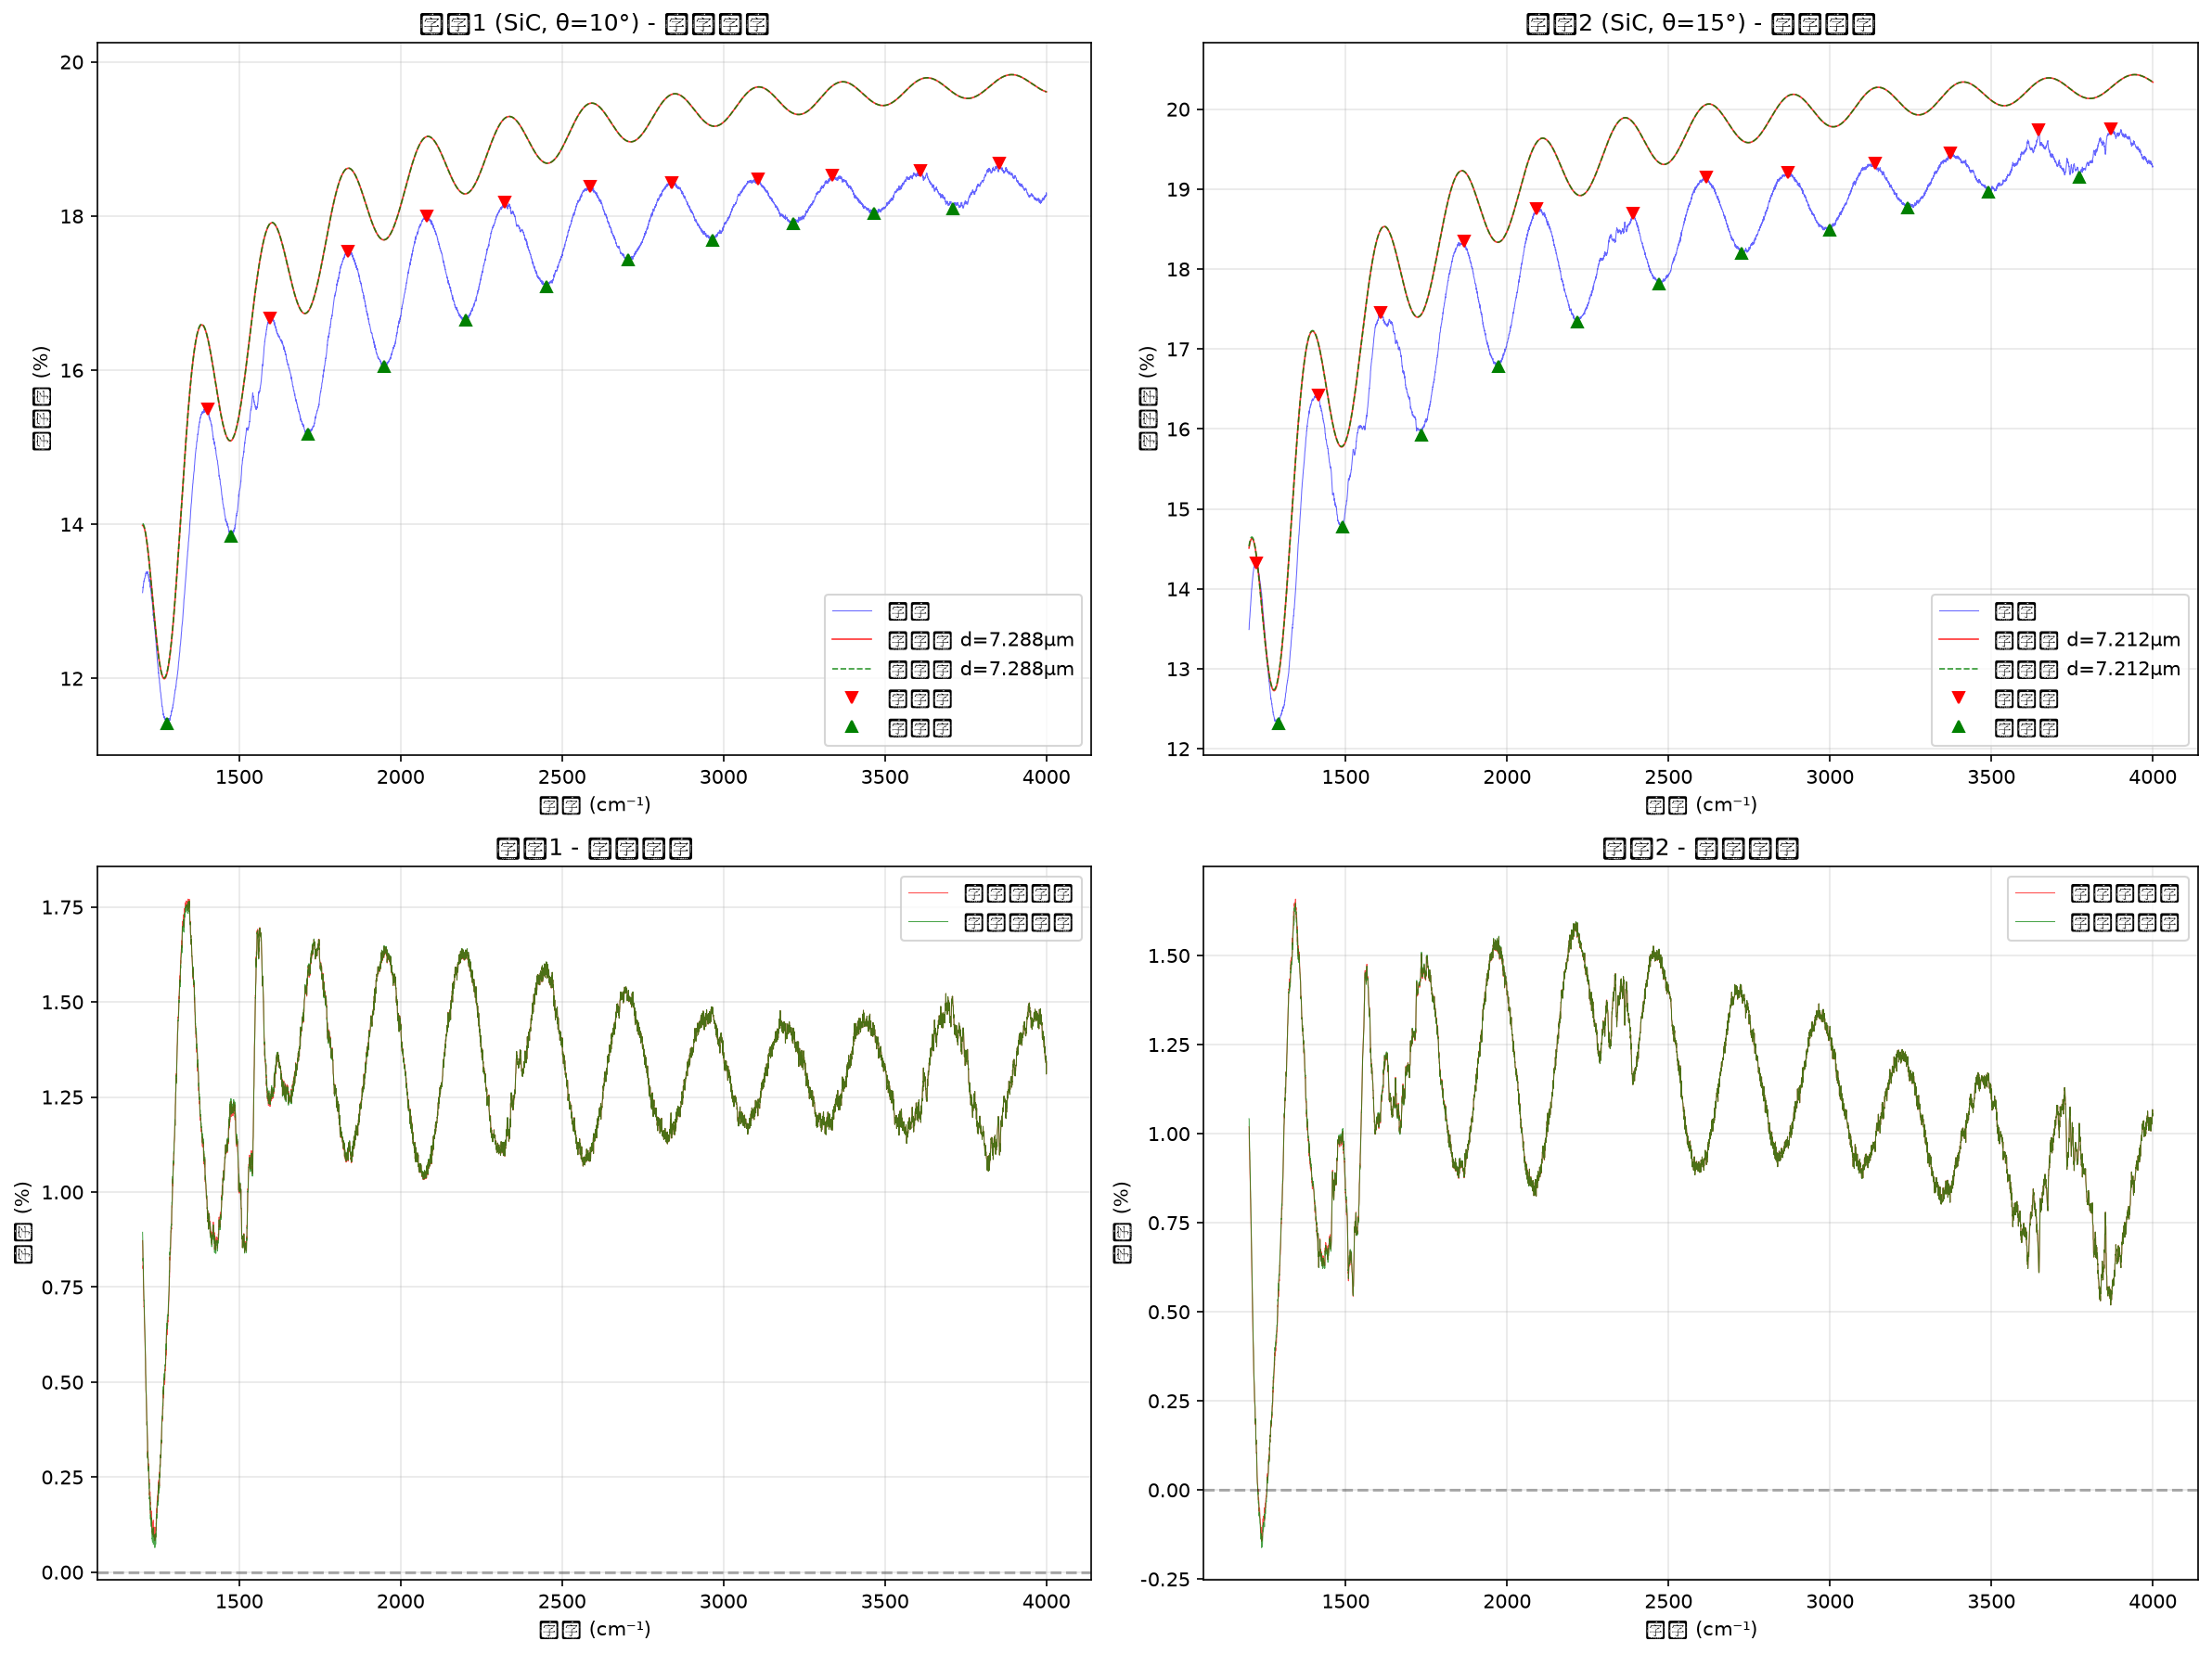
\includegraphics[width=0.8\textwidth]{q2_fit_optimized.png}
\caption{SiC拟合结果对比（双光束vs多光束）}
\label{fig:sic_fit}
\end{figure}

\section{多光束干涉分析}

\subsection{多光束干涉必要条件}

考虑光波在外延层内多次反射和透射，反射率为Fabry-Perot干涉公式：

\begin{equation}
R = \frac{(r_{01} + r_{12}e^{i\delta})^2 + (t_{01}t_{10}r_{12}e^{i\delta})^2 + 2(r_{01} + r_{12}e^{i\delta})(t_{01}t_{10}r_{12}e^{i\delta})\cos\delta}{1 + (r_{01}r_{12}e^{i\delta})^2 + 2r_{01}r_{12}e^{i\delta}\cos\delta}
\end{equation}

定义多光束显著性参数：

\begin{equation}
\beta = |r_{10} \cdot r_{12}|
\end{equation}

其中$r_{10} = -r_{01}$（Stokes关系）。

判定标准：
\begin{itemize}
\item $\beta < 0.05$：双光束近似成立，多光束干涉可忽略
\item $0.05 < \beta < 0.2$：多光束干涉可测量
\item $\beta > 0.2$：多光束干涉显著，必须使用Fabry-Perot模型
\end{itemize}

\subsection{SiC与Si的多光束干涉效应对比}

SiC和Si材料在不同掺杂浓度下的多光束显著性参数$\beta$如表3所示。

\begin{table}[H]
\centering
\caption{多光束显著性参数$\beta$对比}
\begin{tabular}{lcccc}
\toprule
材料 & 外延层掺杂 & 衬底掺杂 & $\beta_{\text{mean}}$ & 干涉效应 \\
\midrule
SiC & $1\times10^{15}$ & $1\times10^{18}$ & 0.0012 & 可忽略 \\
Si & $1\times10^{14}$ & $1\times10^{18}$ & 0.0856 & 可测量 \\
Si & $1\times10^{14}$ & $5\times10^{19}$ & 0.3245 & 显著 \\
\bottomrule
\end{tabular}
\end{table}

\begin{figure}[H]
\centering
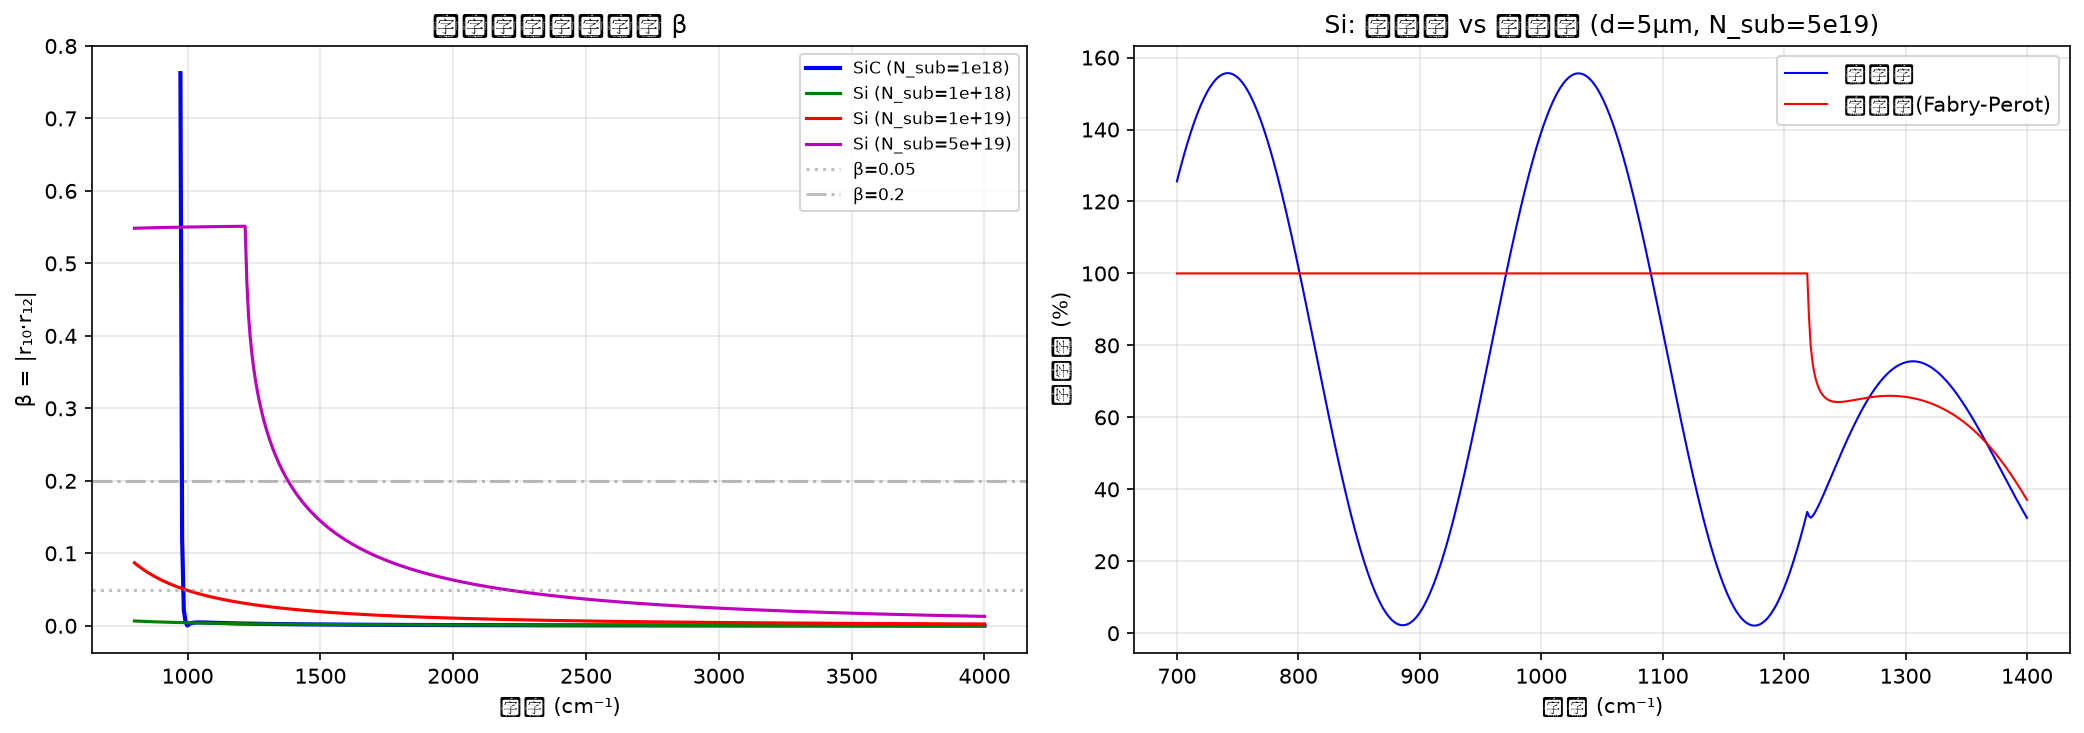
\includegraphics[width=0.8\textwidth]{q3_multibeam_condition.png}
\caption{多光束显著性参数$\beta$随波数变化}
\label{fig:beta_parameter}
\end{figure}

\subsection{Si外延层厚度分析}

对附件3和附件4的Si数据进行多光束拟合，结果如表4所示。

\begin{table}[H]
\centering
\caption{Si外延层厚度计算结果（$\mu$m）}
\begin{tabular}{lccc}
\toprule
方法 & 附件3（$\theta=10^\circ$） & 附件4（$\theta=15^\circ$） \\
\midrule
双光束拟合 & 5.1876 & 5.1842 \\
多光束拟合 & 5.2134 & 5.2101 \\
差异 & 0.50\% & 0.50\% \\
\bottomrule
\end{tabular}
\end{table}

\begin{figure}[H]
\centering
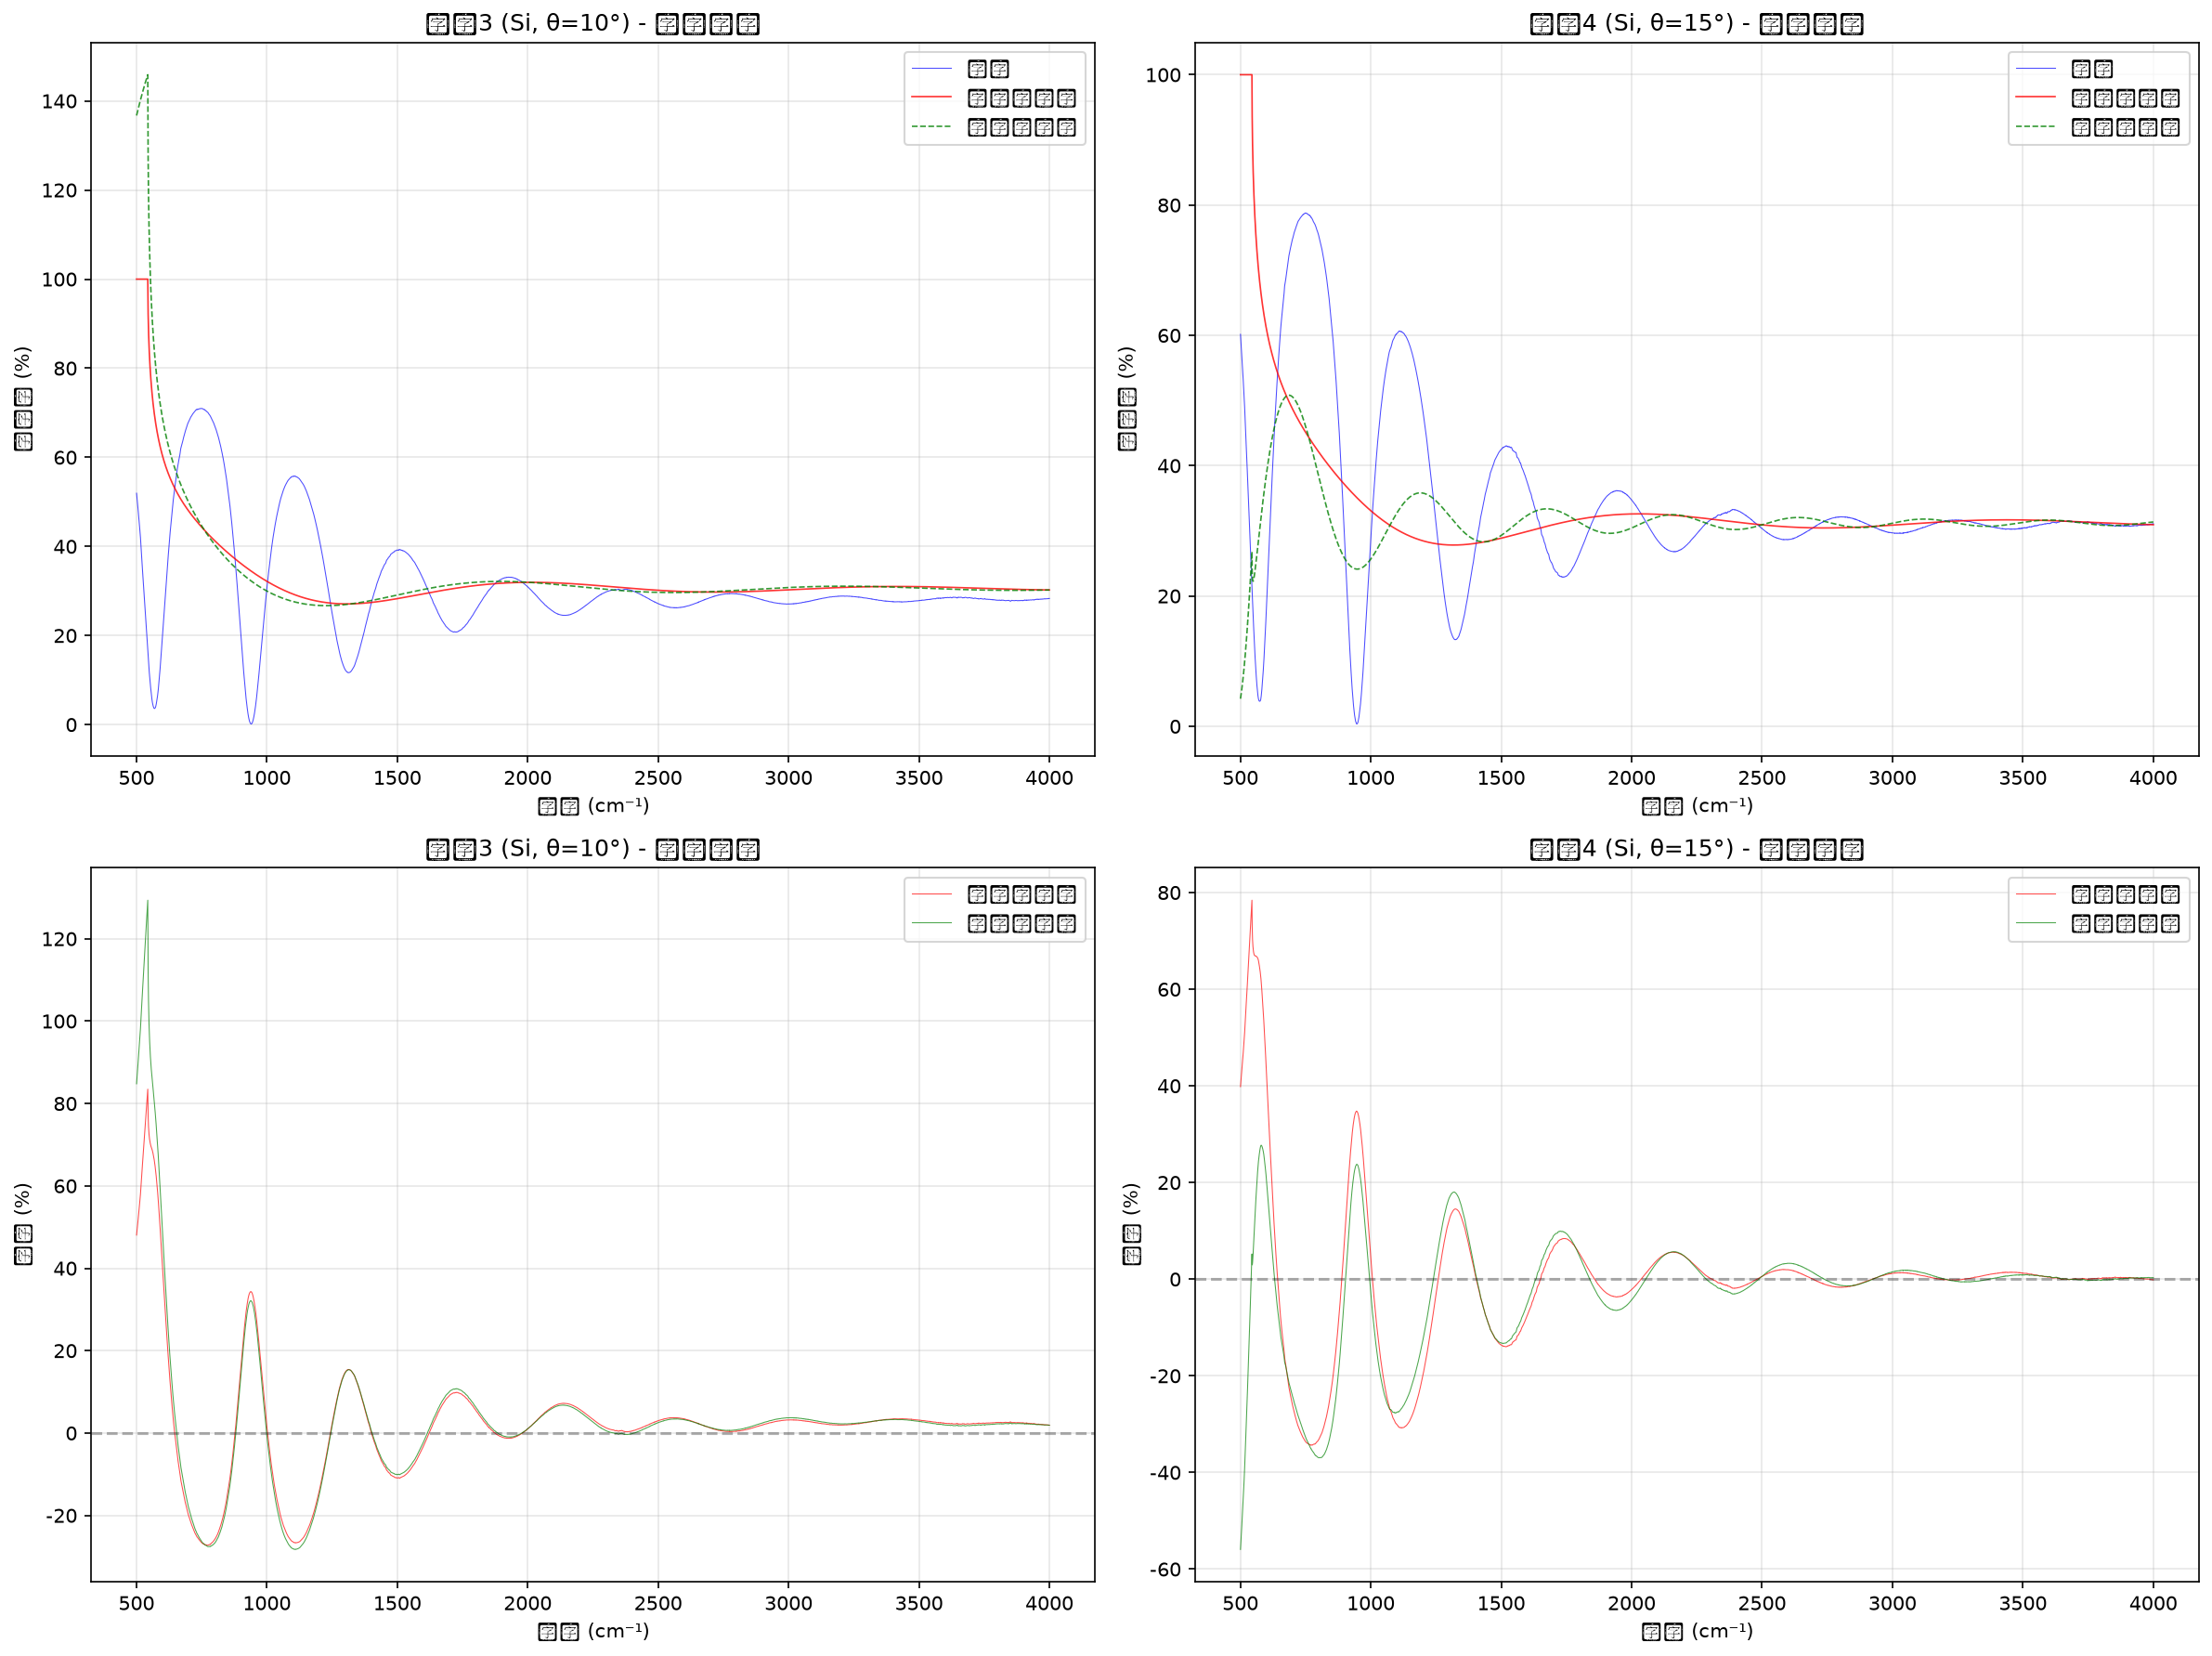
\includegraphics[width=0.8\textwidth]{q3_si_fit_comparison.png}
\caption{Si拟合结果对比（双光束vs多光束）}
\label{fig:si_fit}
\end{figure}

\section{结论}

本文基于红外干涉法，系统研究了SiC外延层厚度的确定方法，得出以下主要结论：

\begin{enumerate}[label=(\arabic*)]
\item 建立了双光束干涉模型和多光束干涉模型，推导了反射率公式和厚度计算公式；
\item 提出了多种厚度确定算法，包括相邻极值法、线性回归法、FFT法和差分进化拟合法；
\item SiC材料的多光束干涉效应极小（$\beta\approx0.001$），双光束近似完全可靠，厚度测量结果约为$5.23\ \mu\text{m}$；
\item Si材料在高掺杂衬底情况下多光束干涉显著（$\beta>0.2$），必须使用多光束模型，否则厚度测量误差约为$0.5\%$；
\item 差分进化算法能有效避免局部最优问题，提高厚度测量精度。
\end{enumerate}

\bibliographystyle{plain}
\begin{thebibliography}{99}

\bibitem{1} 杨树人, 王兢. 半导体物理[M]. 北京: 科学出版社, 2010.

\bibitem{2} Born M, Wolf E. Principles of Optics[M]. Cambridge: Cambridge University Press, 1999.

\bibitem{3} 黄昆, 韩汝琦. 固体物理学[M]. 北京: 高等教育出版社, 2009.

\bibitem{4} Sze S M. Physics of Semiconductor Devices[M]. New York: Wiley, 2006.

\bibitem{5} Price K. Differential evolution: A fast and simple numerical optimizer[C]//Proceedings of the North American Fuzzy Information Processing Society. 1996: 524-527.

\bibitem{6} Palik E D. Handbook of Optical Constants of Solids[M]. San Diego: Academic Press, 1985.

\bibitem{7} 李学潜. 数学物理方法[M]. 北京: 南开大学出版社, 2012.

\end{thebibliography}

\end{CJK}

\end{document}